% !TEX TS-program = pdflatexmk
%header and footer for separate chapter files

\ifx\whole\undefined
\documentclass[12pt, leqno]{book}
\usepackage{graphicx}
\input style-for-curves.sty
\usepackage{hyperref}
\usepackage{showkeys} %This shows the labels.
%\usepackage{SLAG,msribib,local}
%\usepackage{amsmath,amscd,amsthm,amssymb,amsxtra,latexsym,epsfig,epic,graphics}
%\usepackage[matrix,arrow,curve]{xy}
%\usepackage{graphicx}
%\usepackage{diagrams}
%
%%\usepackage{amsrefs}
%%%%%%%%%%%%%%%%%%%%%%%%%%%%%%%%%%%%%%%%%%
%%\textwidth16cm
%%\textheight20cm
%%\topmargin-2cm
%\oddsidemargin.8cm
%\evensidemargin1cm
%
%%%%%%Definitions
%\input preamble.tex
%\input style-for-curves.sty
%\def\TU{{\bf U}}
%\def\AA{{\mathbb A}}
%\def\BB{{\mathbb B}}
%\def\CC{{\mathbb C}}
%\def\QQ{{\mathbb Q}}
%\def\RR{{\mathbb R}}
%\def\facet{{\bf facet}}
%\def\image{{\rm image}}
%\def\cE{{\cal E}}
%\def\cF{{\cal F}}
%\def\cG{{\cal G}}
%\def\cH{{\cal H}}
%\def\cHom{{{\cal H}om}}
%\def\h{{\rm h}}
% \def\bs{{Boij-S\"oderberg{} }}
%
%\makeatletter
%\def\Ddots{\mathinner{\mkern1mu\raise\p@
%\vbox{\kern7\p@\hbox{.}}\mkern2mu
%\raise4\p@\hbox{.}\mkern2mu\raise7\p@\hbox{.}\mkern1mu}}
%\makeatother

%%
%\pagestyle{myheadings}

%\input style-for-curves.tex
%\documentclass{cambridge7A}
%\usepackage{hatcher_revised} 
%\usepackage{3264}
   
\errorcontextlines=1000
%\usepackage{makeidx}
\let\see\relax
\usepackage{makeidx}
\makeindex
% \index{word} in the doc; \index{variety!algebraic} gives variety, algebraic
% PUT a % after each \index{***}

\overfullrule=5pt
\catcode`\@\active
\def@{\mskip1.5mu} %produce a small space in math with an @

\title{Personalities of Curves}
\author{\copyright David Eisenbud and Joe Harris}
%%\includeonly{%
%0-intro,01-ChowRingDogma,02-FirstExamples,03-Grassmannians,04-GeneralGrassmannians
%,05-VectorBundlesAndChernClasses,06-LinesOnHypersurfaces,07-SingularElementsOfLinearSeries,
%08-ParameterSpaces,
%bib
%}

\date{\today}
%%\date{}
%\title{Curves}
%%{\normalsize ***Preliminary Version***}} 
%\author{David Eisenbud and Joe Harris }
%
%\begin{document}

\begin{document}
\maketitle

\pagenumbering{roman}
\setcounter{page}{5}
%\begin{5}
%\end{5}
\pagenumbering{arabic}
\tableofcontents
\fi


\chapter{Scrolls and the Curves They Contain}
\label{ScrollsChapter}


\begin{verbatim}
 The naming of cats is a difficult matter,
 It isn't just one of your everyday games.
 You may think that I am as mad as a hatter,
 When I tell you each cat must have three different names.
 The first is the name that the family use daily ...
 But I tell you, a cat needs a name that's particular ...
 But above and beyond there's still one name left over,  ...
 [his] deep and inscrutable, singular name.
\end{verbatim}
--T. S. Eliot, Old Possum's Book of Practical Cats\footnote{\cite{PracticalCats}}

\section*{}
Some of the simplest subvarieties in projective space are the \emph{rational normal scrolls}. They appear in many contexts in algebraic geometry, and are useful for describing the embeddings of curves of low degree and genus. 

We begin this chapter by giving three different characterizations of these varieties, each useful in a different context: First a classical geometric construction that gives a good picture, then an algebraic description that allows one to ``find" the scrolls containing a given variety, and then a more modern geometric definition that makes it easy to understand the divisors on a scroll. Finally, we turn to some of the applications to the embeddings of curves. We will focus on the 2-dimensional case because this is the case that occurs in our applications.

In this chapter we will refer to rational normal scrolls simply as scrolls. The third characterization we will give lends itself to a natural generalization to  irrational ruled varieties, In the literature the word ``scroll'' is often used for this wider class.

\section{Some classical geometry (the name the family use daily)}\label{daily name}

To construct a scroll of dimension 2 in $\PP^n$, we start by choosing integers $0\leq a_1 \leq a_2$ with $a_1 + a_2 = n-1$, and consider  a pair of complementary linear subspaces $\PP^{a_1}$ and $\PP^{a_2} \subset \PP^n$---that is, we have an $(n+1)$-dimensional vector space $V$, expressed as a direct sum $V = V_1 \oplus V_2$ of subspaces $V_1, V_2 \subset V$ of dimensions $a_1+1$ and $a_2+1$, and let $\PP^{a_1} = \PP V_1$ and $\PP^{a_2} = \PP V_2 \subset \PP V$.

Next, we take $\phi_i : \PP^1 \to \PP^{a_i}$ to be the map given by a basis of homogeneous polynomials of degree $a_i$. (If $a_i > 0$, this is of course the usual parametrization of a rational normal curve $C_i \subset \PP^{a_i}$; if $a_i = 0$ this is just the constant map from $\PP^1$ to a point.) Finally, we define the scroll $S(a_1, a_2)$ to be the union of the lines
$$
S(a_1,a_2) := \bigcup_{t\in \PP^1} \overline{\phi_1(p), \phi_2(p)}.
$$

If $a_1\leq a_2$ we call the curve $C_{a_{1}}$ the \emph{directrix} of the scroll, and we call the lines $ \overline{\phi_1(p), \phi_2(p)}$ the \emph{rulings} of the scroll. For example we can realize a smooth quadric surface in $\PP^3$ as the union $S(1,1)$ of the lines joining corresponding points on two skew lines. 

\fix{Insert picture!}

In the degenerate case $a_{1}= 0$, $C_{0}= \PP^{0}$ is a point, and the surface $S(0,a_{2})$ is the cone
in $\PP^{a_{2}+1}$ over a rational normal curve of degree $a_{2}$. Since $S(0,a_2)$ is singular when $a_2\geq 2$, it is useful to consider the surface
$$
\tilde S(0, a_2) := \left\{ (t, q) \in \PP^1 \times \PP^n  \mid q \in \overline{\phi_1(t), \phi_2(t)}\right)\}.
$$
This is the blow-up of the cone $S(0, a_2)$ at its vertex; like the surfaces $S(a_1,a_2)$ with $a_1 > 0$ it is a $\PP^1$ bundle over $\PP^1$ and thus is smooth. As we shall see, it is isomorphic to the scroll $S(1, a_2+1)$.

It is not hard to prove directly that $S(a_1,a_2)$ is an algebraic variety, and we shall soon write down its defining equations.


]
From the description above we can immediately deduce the dimension and degree of a scroll:

\begin{proposition}
\begin{enumerate}
\item $S(a_1,a_2)$ is a nondegenerate surface.
 \item $S(a_1,a_2)$ has degree $a_1+a_2$, and codimension $a_1+a_2-1.$
 \item $S(a_{1},a_{2})$ is non-singular if $0<a_{1}, a_{2}$.
 \end{enumerate}
\end{proposition}\label{deg and codim}

\begin{proof}
 The rational normal curves separately span the spaces $\PP^{a_i}$, so a hyperplane containing both of them would contain $\overline{\PP^{a_1}, \PP^{a_{2}}} = \PP$, proving nondegeneracy. 
 
 It is clear from our description that $S$ is 2-dimensional, and thus of
codimension $a_{1}+a_{2}+1 -2 = a_{1}+a_{2}-1$. 

To compute the degree, we choose a general hyperplane $H$ containing $\PP^{a_{1}}$. The intersection $H\cap C_{2}$ consists of $a_{2}$ reduced points. Thus the intersection $H\cap S$ consists of $C_{1}$ and the $a_{2}$ reduced lines connecting 
the points of $H\cap C_{2}$ with their corresponding points on $C_{1}$; this union has degree $a_{1}+a_{2}$.

If $0< a_{1}$ we also see from this argument that, given any point  $p\in S(a_{1},a_{2})$, there is
a hyperplane section that is non-singular at $p$, and thus $S(a_{1},a_{2})$ is nonsingular at $p$.
\end{proof}

A completely parallel construction creates rational normal scrolls of dimension $r$. Start with a series of integers $0 \leq a_1 \leq \dots \leq a_r$;
set $N = \sum_{i=1}^{r}(a_{i}+1)$,  and
decompose $\CC^{N}$ as
$$
\CC^{N} = \bigoplus_{i=1}^{r}\CC^{a_{i}+1}.
$$
Let $\PP^{a_{i}}\subset \PP^{N-1}$ be the subspaces corresponding to the summands,  choose
maps $\phi_i : \PP^1 \to \PP^{a_{i}}$ be a map given by a basis of homogeneous polynomials of degree $a_i$, and define the scroll $S \subset \PP^{N-1}$ by
$$
S:=S(a_{1}, \dots, a_{r}) = \bigcup_{p\in C_{1}}\overline{\phi_1(p), \phi_{2}(p), \dots, \phi_{r}(p)}.
$$
The variety $S$ is nondegenerate of codimension $N-1-r$ and degree $\sum a_{i} = N-r$. The proof is similar to the one we gave for $r=2$.

%As in the surface case, if one or more of the indices $a_i$ are equal to 0, the resulting variety $S$ is a cone. In these cases, it is again useful in some settings to introduce the blow-up of this cone along its vertex, which we can realize as the variety
%$$
%\tilde S := \left\{ (t, q) \in \PP^1 \times \PP^n  \mid q \in \overline{\phi_1(t), \dots, \phi_r(t)}\right)\}.
%$$

To put this construction in context, we recall an elementary fact of projective geometry:
 
\begin{proposition}\label{minimal degree}
 Any irreducible, nondegenerate variety of codimension $c$ in $\PP^{N}$ has degree $\geq c +1$.
\end{proposition}

\begin{proof} We do induction on $c$. The case $c=0$ being trivial,
 we may assume that $c\geq1$. A general plane $L\subset \PP^{N}$ of dimension $c$ meets $X$ in $\deg X$
 distinct general points, which must be nonsingular points of $X$.
 
Let $p\in L\cap X$ be a point. If every secant to $X$ through $p$ lies entirely in $X$, then $X$ is a cone over $p$; but since $p$ was a general point, this would imply that $X$ is a linear space, contradicting non-degeneracy. 

It follows that the projection $\pi_{p}:X \to \PP^{N-1}$ is a generically finite (rational) map from $X$ to $X' := \pi_{p}(X)$,
and thus $\dim X' = \dim X$ and $\codim X' = \codim X-1$. The plane 
$\pi_{p}(L)$ meets $X'$ in the images of the points of $L\cap X$ other than $p$, so
$\deg X\geq \deg X'+1$. By induction, $\deg X' \geq \codim X'+1 = \codim X$, completing the argument.
\end{proof}

Thus scrolls are \emph{varieties of minimal degree}. The reader already knows that the rational normal curves of degree $a$ in $\PP^{a}$ are the only irreducible, nondegenerate curves of degree $a$ and codimension $a-1$. A celebrated theorem of del Pezzo (for surfaces) and Bertini (in general) generalizes this statement:

\begin{fact}\label{classification of scrolls} 
Any irreducible, nondegenerate variety $X\subset \PP^{N}$  with $\deg X = \codim X+1$, is either a quadric hypersurface, a scroll, the Veronese surface in $\PP^{5}$, or a cone over the Veronese surface.
\end{fact}

A proof may be found in \cite{Eisenbud-Harris-Centennial}.

One interesting way to view the construction above is that we chose subvarieties $C_{i}\subset \PP^{a_{i}}$ and a one-to-one correspondence between them, that is, a subscheme
$\Gamma\subset \prod_{i}C_{i}$ that projects isomorphically onto each $C_{i}$; the scroll is then the
union of the planes spanned by sets of points $p_{i}\in C_{i}$ that are ``in correspondence''. There are other interesting varieties constructed starting with other choices of subvarieties $C_{i}$ and subschemes---not necessarily reduced---of $\prod_{i}C_{i}$. See \cite{Eisenbud-Sammartano} for an exploration of this idea.

We tend to speak of ``the'' rational normal scroll rather than ``a'' rational normal scroll'', despite the choices made in the definition, for the following reason:

\begin{proposition}\label{uniqueness of scrolls}
The scroll $S(a_1,a_2)$ is, up to a linear automorphism of $\PP^{a_1+a_2+1}$, independent of the choices made in its
 definition. 
\end{proposition}

\begin{proof} 
To simplify the notation, set $S := S(a_{1}, a_{2})$ and $\PP := \PP^{a_1+a_2+1}$.
To construct $S$ we chose 
\begin{enumerate}
 \item disjoint subspaces $\PP^{a_i}\subset \PP$;
 \item a rational normal curve in each subspace; and
 \item an isomorphism between these curves.
\end{enumerate}
Elementary linear algebra shows that there are automorphisms of $\PP$ carrying any choice of disjoint subspaces to any other choice. Further, since the rational normal curve of degree $a$ is unique up to an automorphism of $\PP^{a}$, the choice in (2) can be undone by a linear automorphism. Finally, any automorphism of $C_{a_{2}}\cong \PP^{1}$ extends to an automorphism of $\PP^{a_{2}} = |\cO_{\PP^{1}}(a_{2})|$, and this extends to an automorphism of $\PP$ fixing $\PP^{a_{1}}$ pointwise,
showing that $S(a_{1}, a_{2})$ is independent, up to an automorphism of the ambient space, of the choice in (3)  as well.
\end{proof}



\section{1-generic matrices and the equations of scrolls
(the name that's particular)}\label{particular name}

Suppose that $X \subset \PP^n$ is embedded by a complete linear series, and that
$\sO_X(1)$ can be ``factored'' as a tensor product $\sL\otimes \sM$ of invertible sheaves. If we pick sets of $p$ independent elements $\{\ell_i\}\subset H^0(\sL)$ and  $q$ independent elements $\{m_i\} \subset H^0(\sM)$ then the multiplication map 
$$
\mu: H^0(\sL) \otimes H^0(\sM) \to H^0(\sO_{\PP^n}(1))
$$
 gives rise to 
a $p\times q$ matrix $M_\mu$ of linear forms on $\PP^n$ whose $i,j$ entry is $\mu(\ell_im_j)$.
More abstractly, we are using the adjunction isomorphism of vector spaces
to identify a map $\mu: A\otimes B \to C$ with a map $A \to Hom(B,C)$.

Regarding the sections of invertible sheaves as rational functions on $X$, we see from the commutativity of
multiplication that the $2\times 2$ minors
of 
$$
\det \begin{pmatrix}
\ell_{i_1}m_{j_1} & \ell_{i_1}m_{j_2}\\
\ell_{i_2}m_{j_1} &\ell_{i_2}m_{j_2}  
\end{pmatrix},
$$
vanish on $X$---that is, the ideal of $2\times 2$ minors $I_2(M_\mu)$ is contained in the homogeneous ideal
of $X$. 
We will see that, if $p=2$, then the ideal $I_2(M_\mu)$
is the ideal of a rational normal scroll of codimension $q-1$.

For example, the rational normal curve $C_a\subset \PP^a$ is $X = \PP^1$ embedded by the complete
linear series $|\sO_{\PP^n}(a)|$, and $\sO_{\PP^1}(a) = \sO_{\PP^1}(1)\otimes \sO_{\PP^1}(a-1)$, 
giving rise to the $2\times a$ matrix
$$
M_\mu := 
\begin{pmatrix}
x_0&x_1&\dots&x_{a-1}\\
x_1&\dots&x_{a-1}&x_a
\end{pmatrix}.
$$
When restricted to $\PP^1$, this becomes
$$
M_a = \bordermatrix{
& s^{a-1}&s^{a-2}t&\dots&t^{a-1}\cr
s&  s^{a}& s^{a-1}t&\dots&st^{a-1}\cr
t&  s^{a-1}t& s^{a-2}t^{2}&\dots&t^{a}\cr
}$$
where we have written $s,t$ for the basis of $H^)(\sO_{\PP^1}(1))$, and bordered the matrix
with the corresponding bases of $H^0(\sO_{\PP^1}(1))$ and $H^0(\sO_{\PP^1}(a-1))$, and it is obvious
that the minors of $M_a$ are 0.

By a \emph{generalized row} of $M_{a}$, we mean a $\CC$-linear combination of the given rows of $M_{a}$. Note that the points at which the $2\times 2$ minors of $M_{a}$ vanish are the points at which the evaluations of the two rows are linearly dependent; that is, the points at which some
generalized row of $M_{a}$ vanishes identically. From Proposition~\ref{RNC generators}, we see that the points of the rational normal curve are exactly the points where all the linear forms in some generalized row
of $M_{a}$ vanish.

%\fix{moving exercise RNC generators to be Proposition ~\ref{RNC generators} in the first section of Ch 3-Curves of genus 0 and 1}
%\begin{exercise}\label{RNC generators} Prove that the homogeneous ideal of $C_a$
% is generated by the
% $2\times 2$ minors of $M_{a}$ by showing:
% 
%\begin{enumerate}
% \item Modulo the 2x2 minors of $M_\mu$
% every monomial in $x_0,\dots, x_a$ can be reduced to the form 
% $$
% x_0^ix_1^{\epsilon_1}\cdots x_{a-1}^{\epsilon_{a-1}}x_a^j\leqno(*)
% $$
% where each $\epsilon_i$ has the value 0 or 1.
% \item Every monomial in $s,t$ can be represented by one
% and only one monomial of the form (*) after setting $x_i := s^{a-i}t^i$.
%\end{enumerate}
% \end{exercise}
% 
The matrix $M_{\mu}$ shares some properties with the generic $p\times q$ matrix because
it is 1-generic in the following sense:

\begin{definition}
 A matrix of linear forms $M$ is  \emph{1-generic} if every generalized row of $M$
 consists of $\CC$-linearly independent forms.. 
 \end{definition}

 For example, the matrix 
$$
M = \begin{pmatrix}
 x &y\\
 z&x
\end{pmatrix}
$$
over $\CC[x,y,z]$ is  1-generic, since if a row and column transformation produced a 0 the determinant would be a product of linear forms, whereas
$\det M = x^2-yz$ is irreducible. 

On the other hand, the matrix
$$
M' = \begin{pmatrix}
 x &y\\
 -y&x
\end{pmatrix}
$$
over $\CC[x,y]$ is not 1-generic, since
$$
\begin{pmatrix}
1&0\\
-i&1 
\end{pmatrix}
M'
\begin{pmatrix}
 1&0\\
 i&1
\end{pmatrix}
= 
\begin{pmatrix}
 x+iy&0\\
 0&x-iy
\end{pmatrix}
$$
(but note that it would be 1-generic if we restricted scalars to $\RR$---thus the definition depends on the field).

Here is another way of seeing that $M'$ above is \emph{not} 1-generic:

\begin{lemma}\label{variables needed}
  \label{size of 1-generic} There exist 1-generic $p\times q$ matrices of linear forms in $n+1$ variables over $\CC$ if and only if $n\geq p+q$.
In particular, the dimension of the space of linear forms spanned by the entries of a  1-generic matrix $M$ of size $p\times q$ is at least $p+q-1$. Moreover, if this space of linear forms has dimension $>p+q-1$, then the restriction of $M$ to a general hyperplane is still 1-generic.
\end{lemma}
\begin{proof} Consider any map of vector spaces $A\otimes B \to C$, where we regard $C$ as a 
space of linear forms.
With notation as above, if $\ell_i\otimes m_j\in \ker \mu$, then the $i,j$ entry of $M_\mu$ is 0 and similarly for
any rank one element $\ell\otimes m\in A\otimes B$. Thus $M_\mu$ is 1-generic if and only if the linear subspace
$\ker \mu \subset  A\otimes B$
is disjoint from the set of rank 1 matrices. This set has codimension $(m-1)(n-1) = mn-m-n+1$,
so for 1-genericity we must have $\codim \ker \mu \geq m+n-1$. Since $\codim \ker \mu = \dim \im \mu\subset C$ we see that any 1-generic matrix must involve at least $m-n+1$ variables. 

Furthermore, the restriction of $M_\mu$ to a hyperplane corresponds to the composite homomorphism
$A\otimes B \to C \to C/\langle x \rangle$, or equivalently to the addition of 1 element to $\ker \mu$, and thus
if $M_\mu$ is 1-generic and involves $>m+n-1$ variables, then the restriction to a general hyperplane
is again 1-generic.
\end{proof}

%\begin{proof}
%If we think of a polynomial ring $\CC[z_0,\dots,z_n]$ as the symmetric algebra
%of a vector space $V$ of rank $n+1$, then we may regard a $p\times q$ matrix of
%linear forms $M$ as coming from a map $m: \CC^{p}\otimes \CC^{q}\to V$. The matrix is 1-generic
%if and only if no ``pure'' tensor $r\otimes s$ goes to zero, that is, iff the kernel $K$ of $m$ intersects the cone of
%pure tensors only in 0. The cone of pure tensors is the cone over the Segre embedding of $\PP^{p-1}\times \PP^{q-1}$, 
%and thus has dimension $(p-1)+(q-1)+1$. Thus a general subspace $K$ of codimension $\geq p+q-1$ will intersect the cone
%only in 0, but any larger subspace $K$ will intersect the cone non-trivially,  and the first two statements follow.
%
%Moreover, if $K$ is any space of codimension $>p+q-1$ that intersects the cone only in 0, then the general subspace $K'\subset K$
%of dimension one larger still intersects the cone only in 0, proving the last statement.
%\end{proof}

\begin{proposition}\label{some generators}
Let $X$ be
an irreducible, reduced variety, and suppose that $\sL,\sM$ are invertible sheaves on $X$.
The matrix $M_\mu$ coming from the map $\mu:H^0(\sL) \otimes H^0(\sM) \to H^0(\sL\otimes \sM)$
is 1-generic.
\end{proposition}

\begin{proof} Each generalized row of $M_\mu$ has entries of the form $s\cdot H^0(\sM)$,
and these are linearly independent.
\end{proof}

1-generic matrices $M$ of size $2\times a$ are very special, as we shall see. The beginning of the story is the following
codimension calculation of the codimension of the ideal $I_2(M)$ generated by the $2\times 2$ minors of $M$:

\begin{lemma}\label{codim of 2,n 1-generic}
If $M$ is a $2\times a$ matrix of linear forms in $\CC[x_0,\dots, x_n$, and $M$ is 1-generic, then $
and $V(I_2(M))$ is irreducible of codimension $a-1$..
\end{lemma}

\begin{proof}
The algebraic set defined by $I_2(M)$ is the set of points on which a generalized row $r_\lambda, \ \lambda\in \PP^1$ of $M$ vanishes.
Because $M$ is 1-generic, each $V(r_\lambda)$ has codimension $a$. Thus $V(I_2(M))$ is fibered by projective
spaces of dimension $n-a$ over $\PP1$, and is thus irreducible of dimension either $n-a$ or $n-a+1$. In the first
case all the spaces $V(r_\lambda)$  would be equal, contradicting Lemma~\ref{variables needed}.
\end{proof}

\begin{exercise}
Let $M$ be a 1-generic $p\times q$ matrix of linear forms, with $p\leq q$. Show that the codimension of
$I_p(M)$ is $q-p+1$. Hint: imitate the proof of lemma~\ref{codim of 2,n 1-generic}.
\end{exercise}

We have seen in Proposition~\ref{RNC generators} that the ideal of minors of the 1-generic $2\times a$ matrix $M_{a}$ associated to the rational normal curve is a prime ideal of codimension $a-1$ and degree $a$. More generally:

\begin{theorem}\label{1-generic basics} Let $M$ be a 1-generic $2\times a$ matrix of linear forms in $S = \CC[x_0,\dots, x_n]$. 
Let $I = I_2(M)$  be the ideal generated by the $2\times 2$ minors of $M$.
 \begin{enumerate}

\item The ideal $I$ is 
prime and the variety $V = V(I) \subset \PP^n$ has degree $a$ and codimension $a-1$.

\item If $a=n$ then $V(I)$ is a rational normal curve.

\end{theorem}


\fix{I'm stuck for the moment on finding a good proof of the primeness}

\begin{proof} 

In Chapter~\ref{HomologicalChapter} we will construct the Eagon-Northcott complex $EN(M)$. This is a free complex
of length $a-1$, and because the codimension of $I$ is $a-1$ it is a minimal free resolution of $S/I$. 
Since the Hilbert
polynomial is determined by the ranks and twists of the modules in the free resolution, we see that $C$ has
the same degree and codimension as the rational normal curve. Since the projective dimension of $S/I$ is
$a-1 = \codim I$, the ring $S/I$ is Cohen-Macaulay (\cite[***]{Eisenbud1995}). 

(1) By Lemma~\ref{codim 2,n 1-generic) the codimension of $I := I_2(M)$ is $a-1$, so $C = V(I)\subset \PP^a$ is a 1-dimensional.

\fix{why couldn't the radical contain a linear form? Need a good argument for this.}

 and 
if $\ell_1, \ell_2$
are general linear forms, then the the image of $I$ in $\overline S :=S/(\ell_1, \ell_2)$  again has
codimension $a-1$, so the Eagon-Northcott complex $EN(\overline S \otimes M)$ provides a minimal free resolution of the image
of $I$ in $S/(\ell_1, \ell_2)$ as well. It follows that $I \overline S$ is generated by $\binom{a}{2}$
linearly independent quadrics, and since this is the vector space dimension of the degree 2 component
of $\overline S$, we see that modulo $(\ell_1, \ell_2)$ the ideal $I$ is the square of the maximal homogeneous ideal
of $\overline S$. ,

From the exactness of $EN(M)$ it follows that the depth of $S/I$ is 2, and $\ell_1,\ell_2$ is a regular
sequence modulo $I$. It follows that the degree of $C$ is the length of $S/(I, \ell_1, \ell_2) = \overline S/(I \overline S)$.
Since $\overliine S$ is a polynomial ring in $a-1$ variable, this length is $a$. 

Since $S/I$ has depth 2, the ideal $I$ 
is saturated, and since $I$
is generated by quadrics, $V(I)$ is nondegenerate. Since any irreducible, nondegenerate curve of degree $\leq a$ in $\PP^a$
 is a rational normal curve of degree $a$, we see that $I$ must be equal to its radical, and be the prime
 ideal defining a rational normal curve. 
 
 Indeed, the isomorphism $V(I) \to \PP^1$ is given by the sheaf $\coker M: S^a(-1) \to S^2$, an invertible sheaf on $\Proj(S/I)$, and the vector space of 
 sections spanned by the images of the generators of $S^2$. The inverse of this isomorphism is a parametrization of All such curves are conjugate under the action of $PGL_{a+1}$,
 and all parametrization 
 
If $r_\lambda$ is the generalized row correspoonding t The map
 $$
 \PP^1 \ni \lambda  \to V(r_\lambda)and all parametrizations differ by an action of $\PGL_2$ corresponding to row operations, this proves part (1).

Let $\phi: \PP^{1}\to \PP^{N}$ be the parametrization of this rational normal curve, and let
$$
\begin{pmatrix}
 \ell_{0,0},\dots, \ell_{0,a-1}\\
  \ell_{1,0},\dots, \ell_{1,a-1}\\
\end{pmatrix}
$$
 Write $\overline{\ell_{i,j}}$ for the restriction of $\ell_{i,j}$ to $X \cong \PP^{1}$; we thus consider
  $\overline{\ell_{i,j}}$ as a form of degree $a$ in 2 variables. 
 Rechoosing coordinates on $\PP^{1}$, we may assume that the first row vanishes at the point $\phi(0,1)$, and the second row vanishes at $\phi(1,0)$ so that each $\overline{\ell_{0,j}}$ is divisible by $s$ and each $\overline{\ell_{1,j}}$ is divisible by $t$. Since the vector space of forms of degree $a$ divisible by $s$ has dimension $a$, we may, rechoosing coordinates on $\PP^{n}$, assume that $\overline{\ell_{0,i}} = s^{a-i}t^{i}$. It follows that
each $\overline{\ell_{1,i}}$ is divisible by $t$, and that the restriction to $\PP^{1}$ of the second
row is proportional to $(t/s)(s^{a},\dots,st^{a-1}$; thus, after multiplying by a scalar, it will become
equal to $s^{a-1}t,\dots,t^{a}$; that is, the matrix $M$ is equivalent under row and column operations to the matrix $M_{a}$ defined above.


2) We will reduce the case $a<n$ to the case $a=n$. Thus we suppose $a<n$, and let $\ell$ be a general linear form, so that $\ell$ is not contained in any minimal
prime of $I_2(M)$. By induction on $n$, the image of $I$ in $S/(\ell) \cong \CC[x_1, \dots, x_n]$ is a prime
of codimension $a-1$; equivalently, the image of $\ell$ in  $S/I_{2}(M)$ is prime and thus $(\ell)$ contains some mimimal prime $P$ of $S/I_2(M)$. It follows that if $f\in P$ then $f = \ell g$, and since $P$ is prime, $g\in P$. This shows that
$P = \ell P$, whence $P = 0$ by Nakayama's Lemma; that is, $I$ is prime of codimension $a-1$. We also see from the induction
that the degree of $I$ (that is, the degree of $V(I)$) is $a$.

%Since $
%
%in $S/\ell \cong \CC[x_{0},\dots, x_{n-1]}$ is prime of codimension $a-1$. Equivalently, 
%
% and degree $a$ so
%$V(I_{2}(M))$ is irreducible of degree $a$ and codimension $a-1$. It remains to show
%that $I_{2}(M)$ is prime.
%
%It follows from the induction that the image $\overline \ell$ of $\ell$ in
%$R :=  S/I_{2}(M)$  generates a prime ideal containing the
%unique minimal prime $P$ of $R$. 
%Every element $f\in P$ is divisible by $\ell$. If $0\neq f\in P$ is a minimal generator, then $f = \ell f'$, and
%since $\ell\notin P$ we must have $f'\in P$, a contradiction. Thus $P = 0$; that is, $I_{2}(M)$ is
%prime, as required.


(3) If the space spanned by the entries of $M$ has dimension $n>a+1$ then the matrix remains 1-generic modulo a general linear form, and thus we may assume that $n=a+1$. By part (2), if suffices to prove
the result for the matrix $M_a$. If we regrade the polynomial ring, giving the variable $x_i$ degree $i^2$
then the anti-diagonal term of each $2\times 2$ minor has strictly lower degree than the diagonal term.
If the $2\times 2$ minors were linearly dependent, then their lowest degree terms would also be linearly dependent, as one can see by passing to the 
associated graded ring with respect to the new grading. However the lowest degree terms are precisely the ${a\choose 2}$ monomials of degree 2
in the variables $x_1, \dots, x_{a-1}$.
\end{proof}

\begin{fact}
The argument in (3) is usually phrased as a Gr\"obner basis argument. A different proof can be given using the Eagon-Northcott complex, and this
applies more generally to prove the independence of the $p\times p$ minors of any $p\times q$ matrix whose minors generate
an ideal of codimension $q-p+1$, the maximum possible value; see for example~\cite[Theorem ***]{Eisenbud1995}
\end{fact}

\begin{exercise}
Show that if $X\subset \PP^n$ is a projective variety whose homogeneous ideal $I$ contains $m$ independent quadrics, then the ideal of the general hyperplane section of $X$ in $\PP^{n-1}$
contains at least $m$ independent quadrics. Use this to prove that if $X$ has codimension $c$ then $m\leq {c+1\choose 2}$, and that equality holds if and only if
$X$ is a variety of minimal degree (that is, $\deg X = c+1$.)
\end{exercise}

\begin{corollary}\label{equations of scrolls} Let $a_{1}, \dots, a_{r}$ be non-negative integers, and let $N = r-1+\sum_{i=1}^{r} a_{i}$.
The ideal of $S(a_{1},\dots,a_{r})\subset \PP^{N}$ is generated by the $2\times 2$ minors of the matrix
{\footnotesize
$$
\setcounter{MaxMatrixCols}{20}
M = \begin{pmatrix}
x_{1,0}&x_{1,1}&\dots&x_{1, a_{1}-1}&|&x_{2,0}&\dots&x_{2, a_{2}-1}&|&\dots&|&x_{r,0}&\dots&x_{r, a_{r}-1}\\
x_{1,1}&x_{1,2}&\dots&x_{1, a_{1}}.  &|&x_{2,1}&\dots&x_{2, a_{2}}&|&\dots&|&x_{r,1}&\dots&x_{r, a_{r}}
\end{pmatrix}
$$
}
Moreover, the scroll admits a linear projection to each $C_{a_i}$.
\end{corollary}

\begin{proof} We may think of the matrix $M$ as consisting of $r$ blocks, $M_{a_{i}}$ of the form (*). These blocks are 1-generic by Proposition~\ref{some generators}. Since they involve distinct variables, it follows that $M$ is 1-generic. Thus by
Theorem~\ref{}, the ideal $I_{2}(M)$ is prime and of codimension $\sum a_{i}-1$, as is the ideal of the scroll. Thus it suffices to show that the minors of $M$ vanish on the scroll.

Let $C_{i}$ be the rational normal curve in the subspace $\PP^{a_{i}}\subset\PP^{N}$.
As always, the set $V(M)$ is the union of the linear spaces on which generalized rows of $M$ vanish; and each such space is the space spanned by the points in the curves $C_{a_{i}}$ corresponding to the part of that row in the block $M_{a_{i}}$---that is, $V(I_{2}(M))$ is the union of the spans of sets of corresponding points on the $C_{a_{i}}$, as required.
\end{proof}

More is true: 
\begin{fact}
 Every
 1-generic $2 \times N$ matrix of linear forms is equivalent to one of the type shown in
Corollary~\ref{equations of scrolls}, and thus the minors of any 1-generic matrix defines a scroll. 
\end{fact}

\begin{proof}[References]
A $2\times a$ matrix of linear forms in $N+1$ variables may be thought of as a tensor
in $\CC^{2}\otimes \CC^{a}\otimes \CC^{N+1}$, or, equivalently, as an $a\times (N+1)$ matrix of linear forms in 2 variables. This, in turn is equivalent to a \emph{pencil} (that is, a projective line) in the vector space of scalar $a\times (N+1)$ matrices. These were first classified by Kronecker; see 
\cite[Theorems *** and ***]{Gantmacher} for a modern exposition. 
\end{proof}


We have used an important result from commutative algebra.
We say that a matrix of forms is \emph{homogeneous} if the entries $f_{i,j}$ satisfy
$$
\deg f_{i,j} + \deg f_{k,l} = \deg f_{i,l}+\deg f_{k,j} \hbox{ for all } i,j,k,l \hbox{ where this makes sense;}
$$
that is, if the determinant of each $2\times 2$ submatrix is ``naturally'' homogeneous.

\begin{fact}\label{Macaulay's Theorem} Every minimal prime over the ideal $I$ of $p\times p$ minors of a homogeneous $p\times q$ matrix forms has codimension $\leq q-p+1$. If $I$ has codimension $q-p+1$, then it is unmixed---that is, there are no embedded primes---and the $p\times p$ minors are linearly independent over the ground field.
\end{fact}

\begin{proof}[References] \fix{I think we're going to prove this in the free res chapter}
\cite[ Theorem *** ]{Eisenbud1995}
\end{proof}

\begin{exercise}\label{many quadrics}
 If $X \subset \PP^n$ is an irreducible, nondegenerate projective variety of codimension $c$ whose homogeneous ideal
 contains ${c\choose 2}$ independent quadratic forms, then $X$ is a variety of degree $c$.
 
Hint: Let $Y = X \cap H$ be a general hyperplane section of $X$ and consider the restriction map $H^0(\cI_{X/\PP^n}(2)) \to H^0(\cI_{Y/\PP^{n-1}}(2))$; repeat $n-c$ times.
\end{exercise}

\begin{corollary}\label{hyperelliptic and trigonal} Suppose that one of the following holds:
\begin{enumerate}
 \item  $C\subset \PP^n$ is a linearly normal hyperelliptic curve, and  
$$
\{D_\lambda \mid \lambda \in \PP^1\}
$$
are the divisors of the $g^1_2$ on $C$; or

\item $C\subset \PP^{g-1}$ is a trigonal canonical curve, and  
$\{D_\lambda \mid \lambda \in \PP^1\}$
are the divisors of the $\g^1_3$.
\end{enumerate}

The union of the lines spanned by the $D_\lambda$
is a scroll $S(a_1,a_2)$ and $\max\{a_1, a_2\}$ is the maximal number of
$D_\lambda$ that are contained in a single hyperplane.
\end{corollary}

\begin{proof}
Let $\sL$ be the invertible sheaf $\cO_C(D_\lambda)$ corresponding to the $g^1_2$ in case 1 or
the $g_3^1$ in case 2 and let $s_\lambda$ be
the section vanishing on $D_\lambda$. Setting $\sM =  \sL^{-1}\otimes \sO_C(1)$, we see that
$s_\lambda\cdot H^0(\sM) \subset H^0(\sO_C(1)$ is the space of linear forms vanishing on
$D_\lambda$. In both cases, this space is a line: this is obvious in case 1, and follows from the 
geometric Riemann-Roch theorem in case 2. 

These forms make up the
generalized rows of the matrix $M_\mu$ corresponding to the multiplication
$\mu: H^0(\sL)\otimes H^0(\sM) \to H^0(\sO_C(	1))$, we see that the union of the lines is a
scroll $S(a_1,a_2)$ cut out by $I_2(M_\mu)$.

The proof is completed by the more general Proposition~\ref{which scroll}.
\end{proof}

\begin{proposition}\label{which scroll}
Let $S(a_1,a_2)\subset \PP^{a_1+a_2+1}$ be a scroll. The maximal number of rulings contained in
a proper subspace of $ \PP^{a_1+a_2+1}$ is $a_2$.
\end{proposition}

\begin{proof}
We may suppose that $a_1\leq a_2$. A hyperplane containing $C_{a_1}$ meets $C_{a_2}$ in $a_2$
points, and thus contains $a_2$ rulings of the scroll. If $H$ were a hyperplane containg more than $a_2$
rulings, then $H$ would meet each curve $C_{a_i}$ in more than $a_i$ points, and thus $H$ would contain
both these curves, so that $S(a_1,a_2)\subset H$. Since $S(a_1,a_2)$ is nondegenerate, this is impossible.
\end{proof}


\section{Scrolls as Images of Projective Bundles (the deep and inscrutable name)}\label{inscrutable name}

Our third description of scrolls is that they are the images of projective space bundles on $\PP^{1}$ under the map given by the complete series associated to the tautological line bundle; when both $a_{1}$ and $a_{2}$ are strictly positive, we will see that this is an embedding. For simplicity we focus on the 2-dimensional case; the case of a higher dimensional scroll is similar. 

We start from the description of 
$
X:=S(a_{1}, a_{2}),
$
with $0\leq a_{1}, a_{2}$ and not both 0,
as the vanishing locus of the minors of the matrix
$$
\setcounter{MaxMatrixCols}{20}
M:= M_{a_{1}, a_{2}} = 
\begin{pmatrix}
x_{1,0}&x_{1,1}&\dots&x_{1, a_{1}-1}&|&x_{2,0}&\dots&x_{2, a_{1}-1}\\
x_{1,1}&x_{1,2}&\dots&x_{1, a_{1}}.  &|&x_{2,1}&\dots&x_{2, a_{1}}
\end{pmatrix}
$$
of Section~\ref{particular name}. For $p = (s,t) \in \PP^{1}$ we write
$R_{p}$ for the locus where the linear forms in $s$ times the first row plus $t$ times the second row, 
$$
sx_{1,0}+tx_{1,1}, \dots, sx_{2, a_{1}-1}+ tx_{2, a_{1}},
$$
all vanish, so that $R_{p}$ is a ruling of $X$ in $\PP^{N}$


\begin{theorem}\label{scroll as proj}
Let $X = S(a_{1}, a_{2})\subset \PP^{N}$, with $N = a_{1}+a_{2}+1$, and assume $0<a_{1}, a_{2}$. The rulings $R_{p}$ of $X$ are the preimages of points under a morphism $\pi: X\to \PP^{1}$. Furthermore, the line bundle 
$$
\sL := \sO_{\PP^{N}}(1)|_{X}
$$ 
restricts to $\sO_{\PP^{1}}(1)$ on each $R_{p} \cong \PP^{1}$, and the pushforward
$\sE := \pi_{*}\sL$ is isomorphic to 
$\sO_{\PP^{1}}(a_{1})\oplus \sO_{\PP^{1}}(a_{2})$. 

Moreover, $X\cong \PP(\cE)$ and the embedding $X\subset \PP^N$ corresponds to the complete linear series $|\cO_{\PP(\cE)}(1)|$.
\end{theorem} 

In Proposition~\ref{singular scrolls} we will extend this to singular scrolls, showing that the scroll $S(0,a)$, which is the cone over the rational normal curve 
of degree $a$, is the image of $S(1,a+1)$ under a map that blows down the line $C_{1}$.

\begin{proof} We write $M$ for the matrix $M_{a_{1}, a_{2}}$.
Since there are $N+1$ independent entries of $M$ the intersection
of $R_{p}$ with $R_{q}$ is empty when $p\neq q$, so there is at least a set-theoretic map $X\to \PP^{1}$ sending the points of $R_{p}$ to $p$. To see that this is really a morphism, consider the sheaf
$$
\sL = \coker \phi: \sO_{\PP^{N}}(-1)^{a+b} \to \sO_{\PP^{N}}^{2}
$$
given by the matrix $M$. Let $p,q$ be distinct points of $\PP^{1}$ and  let
$\tilde p$ be a point in the ruling $L_p$. Since $L_q$ is disjoint from $L_{p}$, some linear form in the generalized row corresponding to $q$ does not vanish at $p$. Thus
the restriction of $M$ to a neighborhood of the point $p$ is equivalent to the matrix
$$
\begin{pmatrix}
0&0&\dots&0 \\
1&0&\dots&0 
\end{pmatrix}
$$
so $\sL$ becomes free of rank 1 when restricted to this neighborhood; that is, $\sL$ is an invertible sheaf.

The two basis vectors of $\sO_{\PP^{N}}^{2}$ map to two global sections
$\sigma_{1},\sigma_{2}$ of $\sL$. By the argument above these two sections generated $\sL$ locally everywhere on $X$, and indeed $\sigma_{1}$ fails to generate $\sL$ locally precisely at the points where the second row of $M$ vanishes. Thus the linear series
defined by these sections corresponds to a morphism $\pi: X \to \PP^{1}$ whose fibers are exactly the rulings of $X$. 

Because  $L_{p}$ is a linear space, the general hyperplane in $\PP^{N}$
meets $L_{p}$ in a point; that is $\sO_{\PP^{N}}(1)$ restricts to $\sO_{\PP^{1}}(1)$ as claimed.

Since $\sL$ is an invertible sheaf and $X$ is a variety, $\sL$ is flat over $\PP^{1}$. Since the restriction of $\sL$ to each fiber is $\sO_{\PP^{1}}(1)$, which has two global sections, we see that $\sE:= \pi_{*}\sL$ is a vector bundle of rank 2 \cite[Theorem III.12.9]{Hartshorne1977}.
Moreover, since $X\subset \PP^{N}$ is non-degenerate, we see that $\sL$, and therefore also $\sE$, has at least $N+1 = a_{1}+a_{2}+2$ independent global sections. 

Now consider the directrices $C_{i}:= C_{a_{i}}\subset X$.  The restriction
$\pi|_{C_{i}}$ is an isomorphism inverse to the parametrization $\PP^{1} \to C_{i}$, and $\sO_{\PP^{N}}(1)|_{C_{i}}$ pulls back to $\sO_{\PP^{1}}(a_{i})$, so $\pi_{*}(\sL|_{C_i}) = \sO_{\PP^{1}}(a_{i})$. Thus the maps $\sL \to \sL|_{C_{a_{i}}}$
induce maps $\sE = \pi_{*}\sL \to \pi_{*}( \sL|_{C_i})$. Putting this together, we get a map
$$
\sE \to \sO_{\PP^{1}}(a_{1}) \oplus \sO_{\PP^{1}}(a_{2}) =: \sE'.
$$
Since the spaces spanned by $C_{1}$ and $C_{2}$ are complementary, this map of rank 2 vector bundles is an inclusion. Since $\sE'$ has only $a_{1}+a_{2}+2$ independent global sections, and is generated by them, the map is an isomorphism, proving that $\sE \cong \sO_{\PP^{1}}(a_{1}) \oplus \sO_{\PP^{1}}(a_{2})$

It remains to show that $X \cong \PP(\sE)$, embedded by $|\cO_{\PP(\cE)}(1)|$. Maps $\phi: X \to \PP (\sE)$ correspond to surjections 
$\alpha: \pi^* \sE \to \sM$ for some line bundle $\sM$ on $X$ in such a way that $\sM = \phi^*\sO_{\PP(\sE)}(1)$ (after passing to an open
cover of $\PP^1$ the proof is almost the same as in the case of a map to projective space; see \cite[II.7.12]{Hartshorne1977}) . We may take $\alpha$ to be the 
natural map $\pi^*\sE = \pi^*\pi_*\sO_X(1)$, and the corresponding map $\beta$ then makes the diagram
 \newarrow{Eq}{}{=}{=}{=}{}
$$
\begin{diagram}
 X&\rTo^{\phi_{|\sO_{X}(1)|}}&\PP^N\\
\dTo^\beta&&\dEq \\
\PP\sE &\rTo^{\phi_{|\cO_{\PP(\cE)}(1)|}}&\PP^N
\end{diagram}
$$
commute, proving the desired assertion.
\end{proof}
 
\begin{proposition} Suppose that $0<a_1\leq a_2$ and
$\sE = \sO_{\PP^1}(a_1)\oplus \sO_{\PP^1}(a_2)$. Let $\pi: X:= \PP(\sE) \to \PP^1$ be the projection.
The sections $\sigma:\PP^1 \to C\subset X$ of $\pi$---that is, maps $\sigma$ such that $\pi\sigma$ is the identity---then 
correspond to surjections
$\sE \to \sL$ for some line bundle $\sL$ on $\PP^1$. Considering  $X$ as embedded in 
$\PP^{a_1+a_2+1}$, we have $\sL = \sigma^*\sO_C(1)$, so the degree of $C$ is equal
to the degree of $\sL$.

Thus $\pi$ admits a section of degree $e$ as a curve in $\PP^{a_1+a_2+1}$ if and only if
$0<e = a_1$ or $e\geq a_2$.
\end{proposition}

\begin{proof}
Apply \cite[II.7.12]{Hartshorne1977}).
\end{proof}

\section{Curves on a 2-dimensional scroll}\label{curves on scrolls}

\noindent{\bf Notation:} Throughout this section we consider the vector bundle 
$$
\sE = \sO_{\PP^1}(a_1) \oplus\sO_{\PP^1}(a_2)
$$
with $0\leq a_1\leq a_2$ and the 
scroll $ S(a_1, a_2) \subset \PP^N$, where $N = a_1+a_2+1$. This scroll is the image of $X = \PP(\sE)$ by a map that is an isomorphism
if $0<a_1$ and is the blow-down of the $C_1$ if $a_1=0$.  We write $\pi:X \to \PP^1$ for the projection, and
$C_{a_i}\subset X$ for the directrix of degree $a_i$. The degree of $S(a,b)$ is $d := a_1+a_2$.

Our interest in scrolls in this book is primarily for the curves that lie on them.The key is to understand the Picard group and the canonical class. We begin with the nonsingular case.

\begin{theorem}\label{pic of scroll}
\begin{enumerate} Suppose in addition that $a_{1}>0$.

\item The Picard group of $X$ is $\Pic X \cong \ZZ^2$, freely generated by  the class $F$ of a ruling and the class $H$ of a  hyperplane section. 
\item The
intersection form on $\Pic(X)$ is given by
$$
\bordermatrix{\kern 10pt\cdot&F&H\cr
F&0&1\cr
H&1&d
}
$$

\item The canonical class of the scroll is $K := -2H +(d-2)F$, so $K^2 = 8$.

\item The degree of a curve in the class $pH+qF$ is $pd+q$, while its arithmetic genus is
${p\choose 2}d+pq-p-q+1$.

\item The class of $C_{a_1}$
is $H-a_2F$, and the class of $C_{a_2}$ is 
is $H-a_1F$. 
\item If $C \subset \PP^{g-1}$ is a trigonal canonical curve and $X$ is the scroll swept out by the trisecants of $C$, then the class of $C$ is $3H+(4-g)F = H-K$. (Note that in this case we necessarily have $a_1 > 0$.)
\end{enumerate}
\end{theorem}

\begin{proof}
We have 
$$
H^2 = \deg X = a_1+a_2 = d; \quad H.F = \deg F = 1; \quad F^2 = 0
$$
where the last equality follows because any two fibers are linearly equivalent and disjoint.
It follows in particular that $H$ and $F$ are linearly independent.

We next show that $\Pic X$ is generated by $H$ and $F$. If $D$ is any divisor,
then $D' = D - (F.D)H$ meets $F$ in degree 0, and it now suffices to show that $D'\sim aF$ for
some integer $a$.
Since $\sO_X(D')|_F = \sO_F$ for any fiber $F$, we see that
$\pi_*(\sO_X(D'))$ is a torsion-free sheaf on $\PP^1$ whose fiber at each point is one-dimensional, 
so $\sL$ is a line bundle on $\PP^1$.  Possibly replacing $D'$ by $-D'$, and using the fact that
$\pi_*(\sO_X(-D')) = (\pi_*(\sO_X(D'))^{-1}$ we may assume that $\sL$ is globally generated, and it follows that  the natural map of line bundles $\pi^*\sL = \pi^*\pi_* \sO_X(D') \to \sO_X(D') $ is a surjection, whence 
$\sO_X(D') \cong \pi^*\sL$. Thus if $q = \deg \sL$ then
$D' \sim qF$. Note that we could also recover $q$ as $H.D'$. This completes the proof of parts
1 and 2.

To compute the canonical class $K_X = pH+qF$ we use the adjunction formula on the rational curves
$H$ and and $F$. Thus $-2 = (F+K).F = p $ and 
$$
-2 = (H+K).H = d + pd+q = d + (-2)d+q
$$
whence $q = d-2$ as required for part 3.
 
 Part 4 is a direct computation from the adjunction formula.
 
For part 5 we observe that a hyperplane containing $C_{a_1}$ meets $X$ in $C_{a_1}$ plus
$a_2$ rulings; thus $C_{a_1}\sim H-a_2F$.

Finally from the adjunction formula $K_C = (K_X+C)\mid_C$ we see that $H+K$ is the class of
the canonical curve. Moreover, any other curve of the same degree would differ by
a divisor meeting $H$ with multiplicity 0, that is, a divisor of the form $E = p(H-dF)$.
But we would also have to have $(H-K+E).(H+E) = 2g-2$, and a straightforward
computation shows that there is no solution to this equation with $p\neq 0$ and $g>3$.
\end{proof}

Now we can say exactly which classes on the scroll contain curves:

\begin{theorem}\label{where are the curves?} Again, suppose that $0<a_{1}$.
There are reduced  curves in the class $D = pH+qF$ if and only if one of the following holds:

\begin{enumerate}
\item $D\sim qF$; that is, $p=0, q>0$; or
\item $D\sim C_{a_{1}}$; that is, $p=1, q=-a_{2}$; or
\item $p\geq 0$ and $D\cdot C_{a_{1}}> 0$; that is, $q \geq -pa_1.$
\end{enumerate}
In case (3) the linear series $|D|$ is basepoint free. When, in addition, $a_2>a_1$ or $q>-pa_1$ the class $|D|$ contains irreducible smooth curves.
\end{theorem}

Note that in case (1) we have $D^{2} = 0$, because any two fibers of $\pi$ are disjoint; in case (2) we have $D^{2}= a_{1}-a_{2}\leq 0$ and in case (3) we have $D^{2}\geq 0$, and $D^2=0$ only if
$d=2, q = -pa_1$. In particular, no irreducible curve
on $X$ other than $C_{a_1}$ can have negative self-intersection.

\begin{proof}
The existence of smooth curves of types 1 and 2 is obvious; the following result will show that
the ones of type 3 move in a base-point-free linear series. By Bertini's theorem \ref{***} such a series must contain smooth curves unless the associated map factors through a curve, in which case $D^2 = dp^2-2pq = p(pa_1+pa_2 -2 q) = 0$, which implies that $a_2=a_1$ and $q= -pa_1$.

The next result, Theorem~\ref{global sections}, thus completes the proof.
\end{proof}

\begin{theorem}\label{global sections} Again, suppose that $0<a_{1}$.
Suppose that $D$ is a divisor on the scroll $X$ as above. If $D \sim pH+qF$, then 
\begin{align*}
 H^{0}(\sO_{X}(D)) &= H^{0}(\sO_{\PP^{1}}(q) \otimes \Sym^{p} \sE)\\
 &= 
\bigoplus_{0\leq i\leq p}H^{0}\bigl(\sO_{\PP^{1}}(q + (p-i)a_{1}+i a_{2})\bigr).
\end{align*}
and $|D|$ is basepoint free iff every summand is nonzero.
Thus, numerically,
$$
h^{0}(\sO_{X}(D)) = 
%\sum_{\{i\ \mid\ q+(p-i)a_{1}+i a_{2} \geq 0\}}H^{0}\bigl(\sO_{\PP^{1}}(q + (p-i)a_{1}+i a_{2})\bigr)
%= 
\sum_{\{i\ \mid\ q+(p-i)a_{1}+i a_{2} \geq 0\}}1+(q + (p-i)a_{1}+i a_{2}),
$$
and
$|D|$ is base point free iff $p\geq 0$ and $q\geq -pa_{1}$.
\end{theorem}

\begin{proof} First, If $q<-pa_{1}$, then 
$$
D\cdot C_{a_{1}} = (pH+qF) \cdot (H-a_{2}F) = p(a_{1}+a_{2}) -pa_{1}+q = pa_{1}+q < 0.
$$
so any effective divisor in the class of $D$ must have a component in common with $C_{a_{1}}$.

Let $\pi:X\to \PP^{1}$ be the structure map of the projective bundle $X = \PP_{\PP^{1}}(\sE)$.
We have $H^{0}(\sO_{X}(pH+qF)) = H^{0}(\pi_{*}(\sO_{X}(pH+qF)))$. Also, 
We may write $\sO_{X}(pH+qF)$ as $\sO_{X}(p) \otimes \pi^{*}\sO_{\PP^{1}}(q)$, and since
$sO_{\PP^{1}}(q)$ is a line bundle we see that 
$$
\pi_{*}\bigl(\sO_{X}(p) \otimes \pi^{*}\sO_{\PP^{1}}(q)\bigr) 
 = \pi_{*}\bigl(\sO_{X}(p)\bigr)\otimes \sO_{\PP^{1}}(q).
$$

The projective bundle $\PP(\sE)$ is
by definition Proj of the symmetric algebra $\PP(\sE):=\Proj(\Sym(\sE))$. Over any open 
subset $U$ of the base $\PP^1$ over which $\sE$ is free, this is $\pi^{-1}(U) = U\times \PP^2$,
and it follows that $\pi_*(\sO_{\PP(\sE)}(p)) = \Sym^p\sE$. 
Thus 
\begin{align*}
\pi_{*}(\sO_{X}(pH+qF)) &= 
\pi_{*}\bigl(\sO_{X}(p) \otimes \pi^{*}\sO_{\PP^{1}}(q)\bigr) \\
 &= \pi_{*}\bigl(\sO_{X}(p)\bigr)\otimes \sO_{\PP^{1}}(q)\\
&=  \Sym^{p}(\sE)\otimes \sO_{\PP^{1}}(q)\\
&=  \bigl(\bigoplus_{0\leq i\leq p} \sO_{\PP^{1}}((p-i)a_{1}+i a_{2})\bigr) \otimes \sO_{\PP^{1}}(q),
\end{align*}
and the first formula follows. 

Clearly, every term 
$H^{0}(\bigl(\sO_{\PP^{1}}(q + (p-i)a_{1}+i a_{2})\bigr))$ is nonzero iff and only if 
$H^{0}(\sO_{\PP^{1}}(q + pa_{1})$ is nonzero iff $q\geq -pa_{1}$.
If $\sigma = \sum \sigma_i$ is a section of $\sO_X(D)$ written according to the decomposition
above, then the restriction of $\sigma$ to  the rational normal curve $C_{a_1} = \PP(\sO_{\PP^1}(a_1)$ is the component $\sigma_0$, and similarly for $C_{a_2}$ and $\sigma_p$. Thus when  all the summands are nonzero
there are sections  vanishing on $C_{a_{1}}$ but not $C_{a_{2}}$, and vice versa, so the system is base point free. 
\end{proof}

 
We can easily compute the degrees and genera of curves that lie on scrolls:

\begin{proposition}Again, suppose that $0<a_{1}$.
 Suppose that $D\sim pH+qF$ is a smooth irreducible curve on $S(a_{1}, a_{2})$ as in Theorem~\ref{where are the curves?}. 
\begin{itemize}
 \item The degree of $D$ is $p(a_{1}+a_{2}) +q$.
 \item The genus of $D$ is ${p\choose 2}(a_{1}+a_{2}) + (p-1)(q-1)$.
\end{itemize}
\end{proposition}
  
\begin{proof} The degree of $D$ is $H\cdot D$, yielding the given formula. Let $g$ be the genus of $D$. 
By the adjunction formula
\begin{align*}
2g-2 =  \bigl((p-2)H+&(q+a_{1}+a_{2}-2)F\bigr)\cdot (pH+qF)\\ 
 &= (p^{2}-p)(a_{1}+a_{2})+2(pq-p-q)
\end{align*}
so $g = {p\choose 2}(a_{1}+a_{2}) + (p-1)(q-1)$ as required.
\end{proof}

\begin{exercise}\label{general projections}
Improve the result of Exercise~\ref{special projections} by showing that, if $0\leq a_1,\leq a_2$, then
 the projection of $S(a_1,a_2)$ from any point not on $C_{a_1}$ (or not the vertex, in case $a_1=0$) is 
 is $S(a_1, a_2-1)$.
\end{exercise}
\begin{fact}
A general curve $C$ of  genus $\geq 22$ does not lie on any 2-dimensional scroll.
\end{fact}
\begin{proof}
Except when $D\sim C_{a_{1}}$, a rational curve of negative self-intersection, every nonsingular curve on $X$ moves in a non-trivial linear series. However the moduli space of curves of genus $\geq 22$ is of general type, and this implies in particular that there there is no nontrivial rational family of curves containing a general curve of 
genus $\geq 22$. But if the linear series containing $C$ had all nonsingular fibers isomorphic to $C$, then
$X$ would be birationally isomorphic to $C\times \PP^{1}$, and thus not rational, a contradiction.
\end{proof}

\fix{add: hyperelliptic curves; and also divisors on the cone}
\fix{consider an exercise to find the automorphism group}
%\section{Automorphisms} (first compute the intersection form...) \fix{probably drop this section -- seems we don't use it elsewhere.}
%\section{Appendix: Centennial Account}

Finally, we treat the case of the cone over a rational normal curve:
\begin{proposition}\label{singular scrolls}
If $X$ is a scheme, $\sE$ a locally free sheaf on $X$, and $\sL$ an invertible sheaf on $X$, 
and Let $\pi: \PP(\sE)\to X$ the natural projection.
$$
\PP(\sL \otimes \sE)\cong \PP(\sE).
$$
Under this isomorphism the invertible sheaf $\sO_{\PP(\sE\otimes \sL)}(1)$ corresponds to the invertible sheaf
$\sO_{\PP(\sE)}(1)\otimes \pi^{*}\sL$. 

Moreover, the singular scroll $S(0,a_{2})$, which is the cone over a rational normal curve of degree $a_{2}$, is the image of
$S(1, a_{2}+1)$ under the map corresponding to the complete linear series 
$$
|\sO_{S(1, a_{2}+1)}(1) \otimes \pi^{*}(\sO_{\PP^{1}}(-1))|,
$$
which blows down the line $C_{1}$.
\end{proposition}

Note that $S(1,a_2+1)$ is isomorphic to the surface $\tilde S(0, a_2)$ of Section~\ref{daily name}.

\begin{proof} 
The desired map $\PP(\sE) \to \PP(\sE\otimes \sL)$ corresponds to the surjection 
$\pi^*(\sE \otimes\sL) \ \pi^*(\sE) \otimes \pi^*(\sL) \to \sO_{\PP(\sE)}(1) \otimes \pi^*(\sL)$, 
and the inverse map is formed similarly.

When $\sE = \sO_{\PP^1}(a_1)\oplus \sO_{\PP^1}(a_2+1)$ and $a_1 = 1$ the
invertible sheaf
$\sO_{S(a_1, a_{2}+1)}(1) \otimes \pi^{*}(\sO_{\PP^{1}}(-1))$ corresponds to the divisor class $H-F$, which meets $C_{a_1}$  in degree 0, so the image
of $C_{a_1}$ under the corresponding linear series is a point. However the description of  $H^0(\sE)$ in
Theorem~\ref{global sections} shows that the restriction to $F$
is still the complete linear series $|\sO_{\PP^1}(1)|$, and the restriction to $C_{{a_2}+1}\cong \PP^1$
is $|\sO_{\PP^1}(a_2)|$.
\end{proof}

\begin{corollary}\label{curves on a singular scroll}
 The smooth curves that lie on the cone $S(0,a_2)$ with $a_2>1$ are isomorphic to their strict transforms
 on $S(1,a_2+1)$, and on $S(1,a_2+1)$ these lie in the classes $mH-mF$ and $mH-(m-1)F$ for $m\geq 1$, 
 corresponding to a multiple of the hyperplane section on $S(0,a_2)$ or one ruling plus a multiple of the hyperplane section. The latter is a Weil divisor that is not a Cartier divisor on $S(0,a_2)$.
\end{corollary}

\begin{proof}
These are the classes that intersect $C_{a_1}$ in degree 0 or 1.
\end{proof}

\fix{Added from Ch 3. maybe integrate this with the Corollary above?}
Exercise~\ref{F2}
\begin{exercise}\label{curves on cones}
\item If $C \subset S(0, a_2) \subset \PP^{a_2+1}$ is a smooth curve with class $m$ times the hyperplane section (that is, corresponding to a curve on $S(1,a_2+1)$ with class $mH - mF$), show that
$$
\deg(C) = ma_2 \quad \text{and} \quad g(C) = \binom{m}{2}a_2 - m + 1.
$$
\item If $C \subset S(0, a_2) \subset \PP^{a_2+1}$ is a smooth curve with class $m$ times the hyperplane section plus a ruling (that is, corresponding to a curve on $S(1,a_2+1)$ with class $mH - (m-1)F$), show that
$$
\deg(C) = ma_2 + 1 \quad \text{and} \quad g(C) = \binom{m}{2}a_2.
$$
\end{exercise}

In these terms we can also see which classes on a scroll correspond to hyperelliptic or trigonal curves in the way described by Corollary~\ref{hyperelliptic and trigonal}:

\begin{corollary}\label{which class}
In situation 1 of Corollary~\ref{hyperelliptic and trigonal}, the class of $C\subset \PP^n$ on $S(a_1,a_2)$ is
$2H - mF$, where $m =  2n-2 - \deg C$, which is one less than the number of quadrics needed to generated $I_{C/S(a_1,a_2)}$.

In situation 2, the class of $C$ is 
$3H -  mF$ where $m = g-4$, which is one less than the number of degree 3 minimal generators of $I_{C}.$
\end{corollary}

\begin{proof} Write $d=2$ in the first case and $d=3$ in the second.
Since the lines of the scroll are spanned by the $D_\lambda$, they meet $C$ in d points, 
giving the coefficient of $H$. 

The coefficient of $F$ is $d\deg S(a_1,a_2) - \deg C$ in both cases, and 
$\deg S(a_1,a_2)= 1+ \codim  S(a_1,a_2)$. By Theorem~\ref{global sections}, 
$h^0(dH-mF) = m+1$, so $m$ is one less than the number of minimal generators
of $I_{C/S(a_1,a_2)}$. In case 2, the ideal of the canonical curve $C$ is minimally
generated by cubics together with  the quadrics in the ideal of the scroll, completing the proof. \end{proof}

\fix{did we prove the last statement in general in section 4-5-6 or only in special cases? I believe it
follows from Petri's theorem.}

\fix{ The following material currently appears in 9-uniformposition. Shall we include the Castelnuovo argument here?
\begin{exercise}\label{linear bound is sharp}
Let $D \subset \PP^n$ be a rational normal curve. If $\Gamma \subset D$ is any collection of $d$ points on $D$ (or for that matter any subscheme of $D$ of degree $d$) then the Hilbert function of $\Gamma$ is
$$
h_\Gamma(m) = \min\{d, mn+1\}
$$
\end{exercise} 
Castelnuovo in fact proved a converse to this observation:
\begin{fact}
If $d \geq 2n+3$, then any collection of $d$ points in $\PP^n$ in linearly general position with Hilbert function $h_\Gamma(2) = \min\{d, 2n+1\}$ must lie on a rational normal curve (and then $h_\Gamma(m) = \min\{d, mn+1\}$ for all $m$.) See~\cite[Lemma3.9]{MR685427} for a proof.
\fix{reference for Castelnuovo's $2n+3$}
\end{fact}
This was a key ingredient in Castelnuovo's theorem characterizing curves of maximal genus; we'll see how it's applied in Chapter~\ref{ScrollsChapter} \fix{did we include it?}
}

\fix{Revise the following, moved from the genus 4,5 chapter and referred to there}
\begin{exercise} Trigonal curves of genus 5.\label{trigonal genus 5} 
 Returning to the canonical curve $C \subset \PP^4$, suppose that the intersection $X = Q_1 \cap Q_2 \cap Q_3$ of the three quadrics containing $C$ has dimension 2. If $C$ were a component of $X$, then the sum of the degrees of the irreducible components of $X$ would be strictly greater than 8, which Fulton's theorem doesn't allow. Thus $C$ must be contained in a 2-dimensional irreducible component  $S$ of $X$, and this surface $S$ is necessarily nondegenerate. 

 a rational normal scroll in $\PP^4$ is either
 the union of the lines joining corresponding points on a line and a conic contained in a complementary plane, denoted $S(1,2)$, or the cone over a twisted cubic curve in $\PP^3$, denoted $S(0,3)$. The latter case does not occur here, because by Corollary~\ref{curves on a singular scroll} the smooth curves on $S(0,3)$ are either hypersurface sections, and thus of degree $3$ for
some integer $a$, or in the rational equivalence class of a hypersurface section plus one line,
of degree $3a+1$, and thus not of degree 8. One can see this directly too: if the scroll were the cone over
a twisted cubic, then the lines on the cone would cut out the $g^1_3$ on $C$. Since a pair of lines on the cone span
only a 2-plane, the sum $D$ of the two divisors would be a divisor of degree 6  and thus $K-D$ would be a $g^1_2$, 
so the curve would be hyperelliptic.

In the case when $C$ lies on $S := S(1,2)$, we may write the class of $C$ in terms of the hyperplane class $H$ and the class $F$ of a ruling, $C\sim pH+qF$, and we see from the 
projection of $S$ to $\PP^1$ that $C$ admits
a degree $p$ covering of $\PP^1$. Since we have assumed that $C$ is not hyperelliptic,
we must have $p\geq 3$. By Theorem~\ref{where are teh curves?} we must have
$q\geq -p$. Since $\deg C = C\cdot H = 3p+q = 8$, we must have either 
$C\sim 3H-F$ or $C\sim 4H-4F$. By the adjunction formula, in the second case,
$$
2g(C)-2 = 8 = (C+K_S)\cdot C = (4H-4F)+(-2H+F))\cdot(4H-4F) =4
$$
whereas a similar computation in the first case yields 8; thus $C\sim 3H-F$.

The key thing to note here is that the curve $C$ has intersection number 3 with the lines of the ruling of $S$, meaning that $C$ is a trigonal curve. (We also see that the $g^1_3$ on $C$ is unique: if $D = p + q + r$ is a divisor moving in a pencil, the points $p, q$ and $r$ must lie on a line; since the surface $S$ is the intersection of quadrics, those lines must lie on $S$ and so must be  lines  of the ruling.) We see also that the locus $W^1_4(C)$ has two components: there are pencils with a base point, that is, consisting of the $g^1_3$ plus a base point; and there are the residual series $K_C - g^1_3 - p$. Each of these components of $W^1_4(C)$ is a copy of the curve $C$ itself, and they meet in two points, corresponding to the points of intersection of $C$ with the directrix of the scroll $S$.\fix{why is it clear that there are no others?}
\end{exercise}

\section{Exercises}

\begin{exercise}\label{special projections}
Suppose $1\leq a_1 < a_2$. Show that the projection of $S(a_1,a_2)$ from any point on $C_{a_1}$ is 
$S(a_1-1, a_2)$, and that the projection from any point on $C_{a_2}$ is $S(a_1, a_2-1)$. (If $a_1 = a_2$, projection of $S(a_1,a_2)$ from any point is $S(a_1-1, a_2)$.)

Conclude, in particular, that the blowup of the cone $S(0,a_2)$ over the rational normal curve of degree $a_2$ is $S(1,a_2+1)$.  
\end{exercise}

\begin{exercise}
Show that a matrix $M$ of linear forms is 1-generic iff, even after arbitrary row and column transformations, its entries are all non-zero.
\end{exercise}


%\section{Appendix: Varieties of minimal degree}
%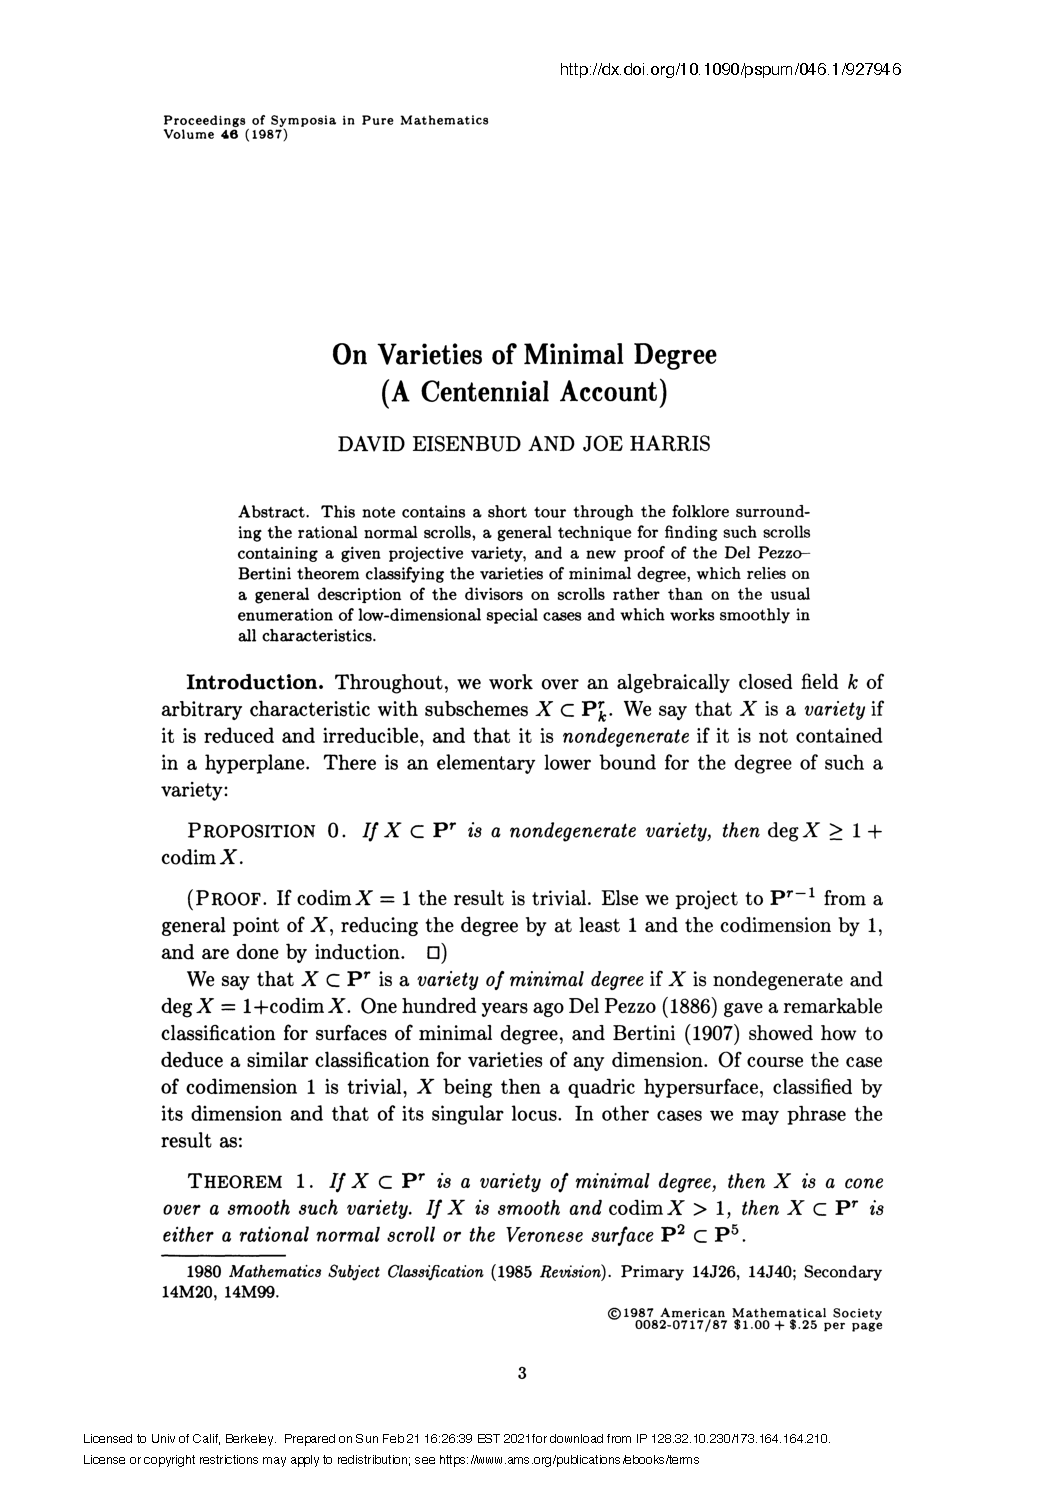
\includepdf[pages=1-11]{Centennial.pdf}


%footer for separate chapter files

\ifx\whole\undefined
%\makeatletter\def\@biblabel#1{#1]}\makeatother
\makeatletter \def\@biblabel#1{\ignorespaces} \makeatother
\bibliographystyle{msribib}
\bibliography{slag}

%%%% EXPLANATIONS:

% f and n
% some authors have all works collected at the end

\begingroup
%\catcode`\^\active
%if ^ is followed by 
% 1:  print f, gobble the following ^ and the next character
% 0:  print n, gobble the following ^
% any other letter: normal subscript
%\makeatletter
%\def^#1{\ifx1#1f\expandafter\@gobbletwo\else
%        \ifx0#1n\expandafter\expandafter\expandafter\@gobble
%        \else\sp{#1}\fi\fi}
%\makeatother
\let\moreadhoc\relax
\def\indexintro{%An author's cited works appear at the end of the
%author's entry; for conventions
%see the List of Citations on page~\pageref{loc}.  
%\smallbreak\noindent
%The letter `f' after a page number indicates a figure, `n' a footnote.
}
\printindex[gen]
\endgroup % end of \catcode
%requires makeindex
\end{document}
\else
\fi


%Let $B= \PP^{1}$, $\sE = \sO_{\PP^{1}}(a_{1}) \oplus \sO_{\PP^{1}}(a_{2})$ and  $\pi: X = \PP_{B}(\sE) \to B$ the structure map.
%
% From the general formula for the Picard group of a projective bundle above, and the fact that the Picard group of
% $\PP^{1}$ is $\ZZ$ we see that the divisor class group of $X$ is the free abelian group on the class of a divisor that belong to $\sO_{X}(1)$, namely the hyperplane section $H$, and $\pi^{*}(\sO_{\PP^{1}}(1)$, namely
% $\pi^{-1}(x)$ for any point $x\in \PP^{1}$, the fiber, proving the first formula.

%
%This is a special case of a very general situation, where, among other things, the Picard group is easy to compute, and which we now explain. 
%
%
%Recall that the projective space $\PP^{n}$ may be defined as $\Proj \Sym_{\CC}(\CC^{n+1})$. The inclusion
%of rings $\CC = \Sym_{\CC}(\CC^{n+1})_{0}\subset \Sym_{\CC}(\CC^{n+1})$ induces a structure map
%$\pi: \PP^{n}\to \Spec \CC$. 
%The variety $\PP^{n}$ comes equipped with a tautological line bundle $\sO_{\PP^{N}}(1)$, which is associated to the graded module $(\Sym_{\CC} \CC^{n+1})(1)$, and a tautological map 
%$$
%\CC^{n+1}\otimes \sO_{\PP^{N}} =\pi^{*}(\CC^{n+1}) \to \sO_{\PP^{N}}(1)
%$$
%that induces an isomorphism on global sections.
%
%\begin{fact}\label{projective space bundles}
%In an exactly parallel way, we may make a projective space bundle $\PP_B(\sE)$ over a variety $B$ from a vector bundle $\sE$ on  $B$ 
%by taking $\PP_B(\sE) = \Proj \Sym_{\sO_{B}} (\sE)$.
%The inclusion of sheaves of rings
%$\sO_{B}  = (\Sym_{\sO_{B}}(\sE))_{0} \hookrightarrow \Sym_{\sO_{B}}(\sE)$ induces a structure map
%$\pi: \PP_B(\sE) \to B$. If $\sE$ has rank $n+1$, then over any closed point $b\in B$ we have
%$\sE_{b} \cong \CC^{n+1}$, and so the fiber $\pi^{-1}(b)$ is $\PP^{N}$. The restriction of 
%$\sO_{\PP_B(\sE)}(1)$ to $\pi^{-1}(b)$ is $\PP^{N}$ is $\sO_{\PP^{N}}(1)$.
%
%The variety $\PP_{B}(\sE)$ comes equipped with a tautological line bundle $\sO_{\PP_{B}}(\sE)(1)$, which is associated to the graded module $(\Sym_{\sO_{B} (\sE)}(1)$, and a tautological map 
%$$
%\pi^{*}(\sE) \to \sO_{\PP_{B}(\sE)}(1)
%$$
%that induces an isomorphism on global sections. Furthermore, 
%$$
%\pi_{*}\sO_{\PP_{B}(\sE)}(p)) = \Sym^{p}(\sE)
%$$
%for every $p$.
%
%Thus the pair $(\PP_{B}(\sE), \sO_{\PP_{B}(\sE)}(1))$ determines $\sE$; but 
%$\PP_{B}(\sE)$ alone determines $\sE$ only up to twisting with a line bundle on $B$. For example, 
%if $\sE$ is itself a line bundle on $B$, then $\PP_{B}(\sE) \cong  B$, but $\sO_{\PP_{B}(\sE)}(1)) \cong \sE$.
%
%Conversely, if $\pi: X\to B$ is a map whose fibers are isomorphic to $\PP^{N}$, and if $X$ carries a line bundle $\sL$ whose restriction to each fiber of $\pi$ is $\sO_{\PP^{N}}(1)$, then $X\cong \PP_{B}(\sE)$ and $\sL \cong \sO_{\PP_{B}(\sE)}(1)$,
%where $\sE = \pi_{*}(\sL)$.
%\end{fact}

%
%Finally, the Picard group of invertible sheaves on $X$ is
%$\Pic X \cong \Pic B \oplus \ZZ h$, where $h$ is the class of the tautological bundle, and
%the map $\Pic B\to \Pic X$ is pull-back by $\pi$.
%The case of scrolls is the case where $B =\PP^{1}$. The situation is simpler than the general case, 
%because every vector bundle
%on $\PP^{1}$ is a sum of line bundles $\sO_{\PP^{1}}(a_{i})$. For simplicity of notation and concreteness, we will concentrate on the case of 2-dimensional scrolls. The case of $r$-dimensional scrolls is exactly parallel, and we give some references. 
% 
%Let $X := S(a_{1}, a_{2})\subset \PP^{N}$ be a nonsingular scroll of degree $a=a_{1}+a_{2}$ and $N = a_{1}+a_{2}+1$. In terms of the geometry of Section~\ref{daily name}, the variety $X$ is fibered over
%$B:=\PP^{1}$ with fibers being the lines joining the corresponding points of the directrices $C_{a_{1}}$ and 
%$C_{a_{2}}$. More precisely, in terms of the algebra of Section~\ref{particular name}, if $M$ is a
%a $2\times a$, 1-generic, matrix of linear forms
%$$
%\begin{pmatrix}
% \ell_0&\ell_{1}&\dots &\ell_{a-1}\\
% \ell_1&\ell_{2}&\dots &\ell_{a}\\ 
%\end{pmatrix}
%$$
% whose $2\times 2$ minors generate the ideal of $X$,
%then the map 
%$$
%\sO_{\PP^{N}}^{a}(-1)\to \sO_{\PP^{N}}^{2}
%$$
% defined by $M$ has rank 1 everywhere
%on $X$, so its cokernel is a line bundle $\sL$ with two global sections. The zero locus
%of the image of the first generator is the set where the second row vanishes, that is, 
%one of the planes of the scroll, and similarly for any scalar linear combination of the
%two generators; that is, $\sL$ defines a morphism $\pi: X \to \PP^{1}$ whose fibers are
%projective lines.
%
%Because the fibers of $\pi$ are embedded as linear spaces, the line bundle $\sO_{\PP^{N}}(1)$
%restricts to a line bundle on each fiber $\PP^{1}$ of $\pi$ that is the  equal to $\sO_{\PP^{1}}(1)$.
%
%
%To check these statements, we reverse the process: Let 
%$\sE =  \sO_{\PP^{1}}(a_{1}) \oplus \sO_{\PP^{1}}(a_{2})$
%and consider the complete linear series  
%$
%|\sO_{\PP_B(\sE)}(1)|.
%$
%Because $\sE$ is generated by global sections, this linear series is base point free and thus defines
%a morphism
%$$
%\phi:  \PP_B(\sE) \to \PP_B(H^{0}(\sE)) = \PP^{N}.
%$$
%
%The variety $\PP_B(\sE)$ contains subvarieties corresponding to the rank 1 quotients 
%$\sO_{\PP^{1}}(a_{i})$ of $\sE$, and the bundle $\sO_{\PP_B(\sE)}(1)$ restricts to
%the bundle $\sO_{\PP_B(\sO_{\PP^{1}}(a_{i}))}(1)$. The sections of $\sO_{\PP^{1}}(a_{i})$ restrict
%as well, and we see that the image of $\phi$ contains the rational normal curves
%$C_{a_{i}}\subset \PP^{a_{i}}$. Since all the sections from $\sO_{\PP^{1}}(a_{1})$ vanish on the $C_{a_{2}}$, and similarly for $\sO_{\PP^{1}}(a_{2})$ and $C_{a_{1}}$, we see that the two curves are embedded in  disjoint subspaces spaces. Furthermore, since the structure maps $C_{a_{i}} = \PP_{B}(\sO(a_{i})) \to \PP^{1}$ are
%isomorphisms, we see that each
% fiber of $\PP_B(\sE)$ meets each $C_{a_{i}}$ in a single point. Thus the embedded
% variety $X\subset \PP^{N}$ is a scroll, as claimed.
%
%
%
%
%Putting this together we have outlined part of the proof of the following:
%
%\begin{fact}\label{push-forward formula}
% If $X := S(a_{1}, a_{2})\subset \PP^{N}$ is a nonsingular rational normal scroll, then
% $X$ is isomorphic to a projective space bundle $\PP_{B}(\sE)$, where $B = \PP^{1}$, and the restriction of $\sO_{\PP^{N}}(1)$ to $X$
% is $\sO_{\PP_B(\sE)}(1)$. Further, writing $\pi: X\to \PP^{1}$ for the structure map, we have
%$$
%\sE = \pi_{*}(\sO_{X}(1)) = \sO_{\PP^{1}}(a_{1}) \oplus sO_{\PP^{1}}(a_{2}),
%$$
%and more generally 
%$$
%\pi_{*}(\sO_{X}(p)) = \Sym^{p}\sE = \sO_{\PP^{1}}(pa_{1}) \oplus \sO_{\PP^{1}}((p-1)a_{1}+a_{2})
%\oplus \cdots\oplus \sO_{\PP^{1}}(pa_{2}).
%$$
%
%\end{fact}
%
%In particular, since $\Pic(\PP^{1}) = \ZZ$, we see that the divisor class group
%of a scroll $S(a_{1}, a_{2})$ is freely generated by the class $H$ of a hyperplane section and the class $F$ of a ruling. The intersection form, is now easy to compute. If $C,D$ are divisor classes on the scroll, we write $C\cdot D\in \ZZ$ for their intersection number.
% 



